\section{Introduction}

\subsection{License and Copyright}

InsightCAE is free software; you can redistribute it and/or modify it under the terms of version 2 of the GNU General Public License\footnote{\url{http://www.gnu.org/licenses/old-licenses/gpl-2.0.html}} as published by the Free Software Foundation. You accept the terms of this license by distributing or using this software.

This manual is Copyright (c) 2017-2021 silentdynamics GmbH.

Permission is granted to copy, distribute and/or modify this document under the terms of the GNU Free Documentation License, Version 1.3 or any later version published by the Free Software Foundation; with no Invariant Sections, no Front-Cover Texts, and no Back-Cover Texts. A copy of the license is included in the section entitled "GNU Free Documentation License".

\subsection{About InsightCAE}

InsightCAE is a framework for building automated analysis and design workflows in Computer-Aided Engineering with a preference for open source tools.

Individual open source projects often meet only subtasks in an analysis process and have very different APIs. To conduct computational tasks, a combination of several software tools is often required. In order to use open source software productive and efficient for everyday tasks, the analysis automation framework InsightCAE was created.

InsightCAE serves as a framework for the implementation of analysis procedures. The objective is to provide adapters and interfaces to the tools and simulation programs that are needed for a specific computing task.

Some common use cases are:
\begin{itemize}
\item create a simulation app

InsightCAE's toolkit library is used to build a simulation app. The workbench or the web interface can be used to present the parameter form to the user and display a 3D preview of the setup. The app generates a result set. InsightCAE contains a viewer to display result sets or compare data from different result sets. The simulation app can be stored in a custom library or in a python script.

\item assist in creation of OpenFOAM cases

InsightCAE contains a GUI (called "Case Builder") to build OpenFOAM cases by putting features together into an OpenFOAM case.

\item build parametric, script-based CAD models

InsightCAE contains an interpreter for script-based CAD models. The underlying CAD kernel is OpenCASCADE (a BREP kernel). 
This can utilized to produce geometry in the course of optimizations, for example.
\end{itemize}

\subsection{Contributors}

The following people have so far contributed to InsightCAE:
\begin{itemize}
\item Hannes Kröger (silentdynamics GmbH)
\item Johann Turnow (silentdynamics GmbH)
%%
%% Please add yourself here, if you made any contribution
%%
\end{itemize}

If you want to get involved in the development, please feel invited to do so!
We greatly appreciate any contribution and we would very much like to add you to the above list.

If you made some modification or addition to the code, which you would like to be merged into the main development line, please consider to send us a pull request\footnote{\url{https://help.github.com/en/github/collaborating-with-issues-and-pull-requests/about-pull-requests}}.

\subsection{Features and Highlights}

InsightCAE's objective is to create automated analysis workflows.
The high level API resides in the core "toolkit" library.
Automated workflows usually involve different external programs and utilities.
For the realization of automated workflows, it is sometimes required, to create add-ons to these external programs.
Thus InsightCAE is also a container for add-ons to other programs.

\begin{itemize}
\item InsightCAD script-based, fully parametric CAD

\begin{itemize}
    \item OpenCASCADE geometry kernel
    \item assemblies, constraint-based sketches, part library, drawing export
\end{itemize}

\item OpenFOAM add-ons (schemes, boundary conditions, models, ...)
\item Pre- \& Postprocessing tool (OpenFOAM Case Builder)
\item analysis workflow automation tools (GUI)
\end{itemize}

\subsection{Reading this Manual}


\subsection{Recommendations for Working with Shell-based Tools in Linux}

Sometimes it is necessary to execute tools in a bash shell, e.g. because no GUI for it is available. And often it is easier to keep an overview in graphical file manager.
Having a console window open together with a file manager window at the same time is an obvious solution but to do so for many cases at a time may easily confuse the desktop. 

Here are two useful hints to solve this issue:
 
\begin{enumerate}

 \item The KDE file manager \textbf{dolphin} offers the possibility to display a console in the lower half of the window (figure \ref{fig:dolphin}). The working directory is synchronized with the directory shown in the graphical window by injection of \textbf{cd} commands. Vice versa, when the working directory is changed in the shell, the graphical display is updated as well.
 
 \begin{figure}[h!]
 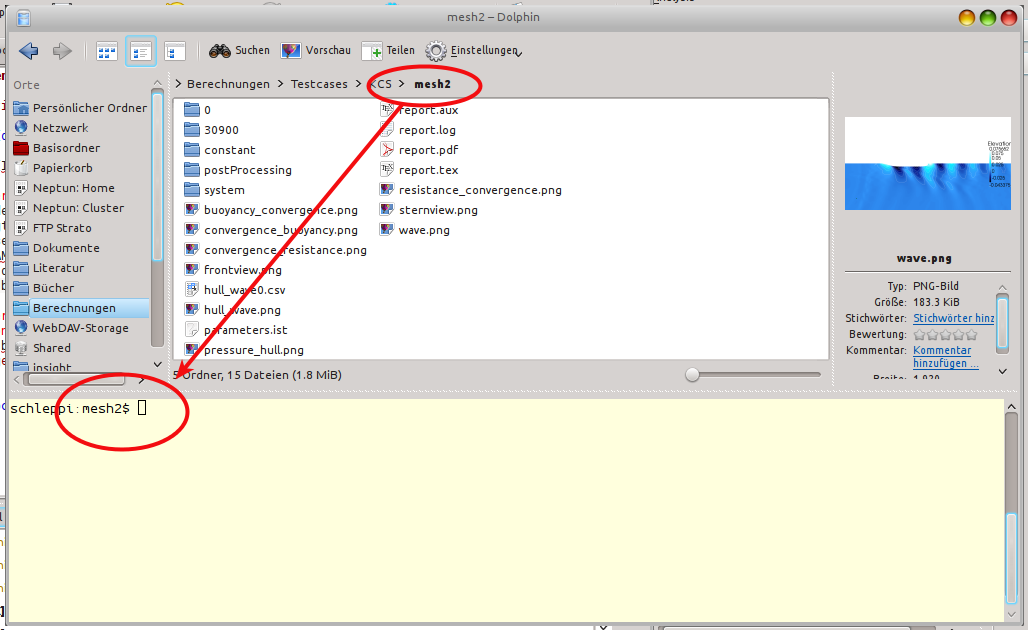
\includegraphics[width=\linewidth]{figs/intro/dolphin_with_terminal} 
 \caption{Dolphin file manager with embedded terminal}
 \label{fig:dolphin}
 \end{figure}

 \item There is a Norton-Commander-like file manager named \textbf{krusader} (figure \ref{fig:krusader}). It offers the same functionality regarding the embedded terminal but a more flexible way of displaying multiple folders. In addition to the two list view on the left and right, multiple tabs for folders can be added in each list view. And there is also a rich interface to define custom commands and file associations.
 
 \begin{figure}[h!]
 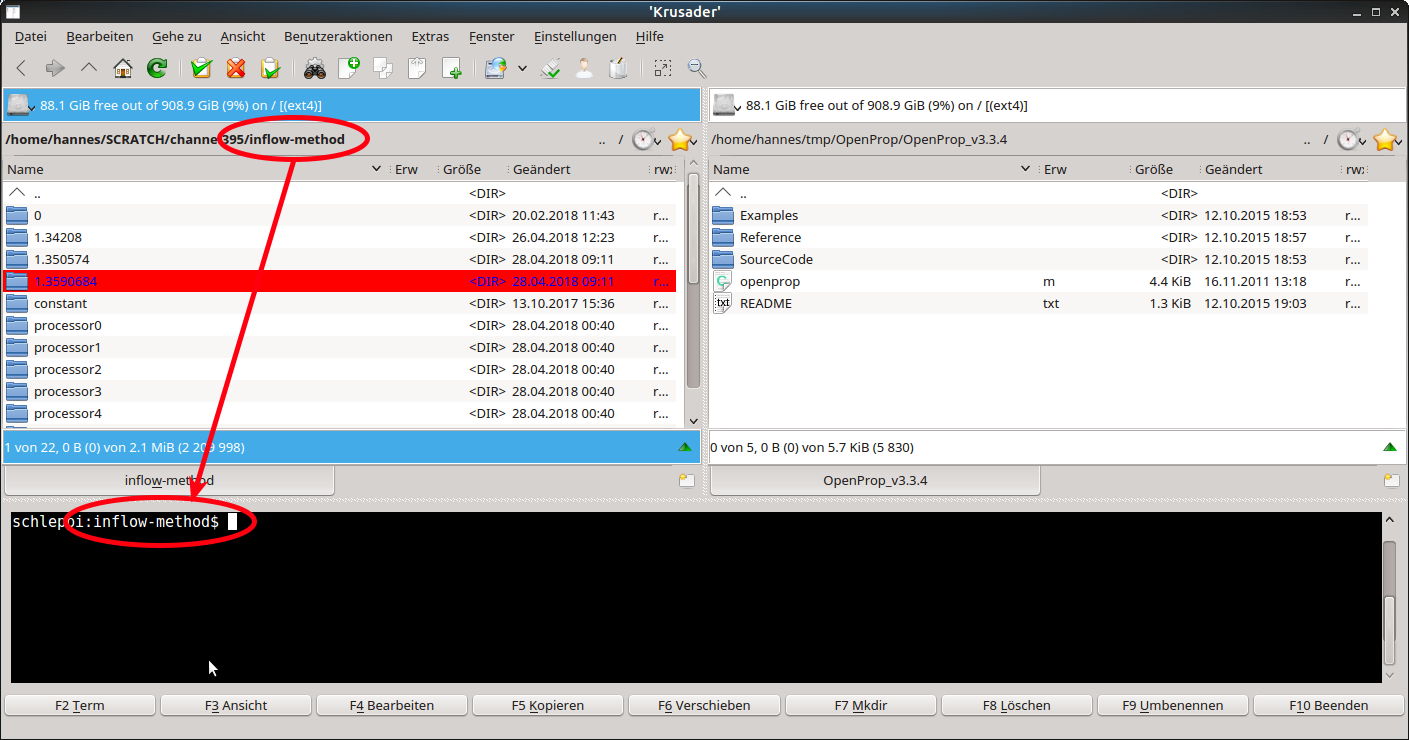
\includegraphics[width=\linewidth]{figs/intro/krusader_with_terminal}
 \caption{Krusader file manager with embedded terminal}
 \label{fig:krusader}
 \end{figure}
 
\end{enumerate}






\section{Additional Sources of Information}

\subsection{In the Web}

\begin{itemize}
\item Source Code Repository \url{https://github.com/hkroeger/insightcae}
\item Issue Tracker \url{https://github.com/hkroeger/insightcae/issues}
\item Web Forum \url{https://groups.google.com/forum/#!forum/insightcae}
\end{itemize}

\subsection{Reporting Bugs and Feature Requests}

Please use the issue tracker \url{https://github.com/hkroeger/insightcae/issues} to report any bugs.

We also monitor the web forum \url{https://groups.google.com/forum/#!forum/insightcae} for questions or feature requests.

\subsection{Getting Professional Help and Support}

Beyond the web resources above, silentdynamics GmbH offers commercial support\footnote{\url{http://silentdynamics.de/en/oss-cae/}} for professional users of InsightCAE. Automated analyses according to customer needs and specifications are implemented  by creating new specialized modules for Insight CAE.
Typical support contracts include also user training and continuous customization and updating of InsightCAE and its add-ons.






\section{Obtaining InsightCAE}

\subsection{Installation using Linux Package Manager}

We provide binary installation packages for Ubuntu-based Linux distributions. We specifically support the latest Ubuntu LTS distibution.

The packages are held in our repository. To install them, first add the silentdynamics apt repository and the associated key by executing:

\begin{lstlisting}[language=bash]
$ sudo apt-key adv --fetch-keys http://downloads.silentdynamics.de/SD_REPOSITORIES_PUBLIC_KEY.gpg
$ sudo add-apt-repository http://downloads.silentdynamics.de/ubuntu
$ sudo apt-get update
\end{lstlisting}

Then, install the community-edition package by executing

\begin{lstlisting}[language=bash]
$ sudo apt-get install insightcae-ce
\end{lstlisting}

Continue with preparing the environment according to section \ref{sec:setupenvironment}

Note: for customers who receive supported, tailored simulation apps from silentdynamics, these apps are bundled into add-ons and the add-ons are included in the installation package.
For each customer, a separate package repository is maintained (with a unique URL, different from the one above) and the name of the installation package is \texttt{insightcae} instead of \texttt{insightcae-ce}.

Note: besides the standard repository at \url{http://downloads.silentdynamics.de/ubuntu} which includes the package built from the "master" branch in the git source code version management system, silentdynamics provides a second package repository with a development package built form the branch "next-release".

\subsection{Installation on Windows}
Our software as well as OpenFOAM and Code\_Aster are currently pure Linux software. 
However, it can also be run under Windows 10 (64 bit only) or later with the help of the "Linux Subsystem for Windows" (WSL).
Virtualization is not used. 
The processes share the memory with the Windows processes and the files are stored in the Windows file system. 

Graphical output from the WSL environment has turned out to be error-prone and poor, thus the software is split into a frontend part, which runs natively in Windows and a backend part which controls the simulation solvers and runs in the WSL environment.
The communication between both is over the network stack.

For the comfortable installation of InsightCAE and OpenFOAM under Windows we provide an installer:

\url{http://downloads.silentdynamics.de/ubuntu_dev/}

The installers for the different versions X.Y.Z are named in the form 

\texttt{InsightCAEInstaller-X.Y.Z.exe}

Note: for customers who receive supported, tailored simulation apps from silentdynamics, the installer is downloaded from the customers dedicated repository URL instead of the one above.

Download the latest EXE file from this link and execute it:

\begin{itemize}
\item It will activate the Windows subsystem for Linux, if it is not already activated
\item The installer bundles the necessary third party programs (ParaView, gnuplot, MiKTeX, Putty)
\item The WSL backend is not immediately created during installation but upon the first start of the workbench GUI.
\item Please note:
\begin{itemize}
\item For the installation, administrator rights are required
\end{itemize}
\end{itemize}

\paragraph{Usage}

Appropriate start menu entries are created.

To complete the setup, perform a system reboot and launch the InsightCAE "Workbench" from the start menu.

Upon the first launch, two things need to be completed:
\begin{enumerate}
\item Set paths to commonly required executables.

The executables are searched and some will not be found since their location is not included in the executable search path environment variable PATH.
If some of the required executables are not found, the configuration dialog shown in figure \ref{fig:set_paths} is brought up.
Click on a row, where no "Path to executable" is printed and click on "Select path...". 
In the dialog box, find the appropriate executable and click "ok".
Repeat this for every executable, which was not found.

\item The presence and the version of the WSL backend is checked.

If there is no WSL existing (as after a fresh install), a message appears and the user should select "Create" to create one.
The form as shown in figure \ref{fig:create_wsl} should appear.

The URL should be properly preset according from which source the installer was downloaded.
For support customers, it is important to enter their credentials into the appropriate fields.

When everything is set, click the button "Ok".
Then the image is downloaded from the server and installed.
The image is approximately 1.5GB so the download takes some time and also the unpacking takes several minutes.
When the creation is done, the creation dialog is closed and the workbench GUI is shown.

\end{enumerate}

\begin{figure}[ht]
\centering
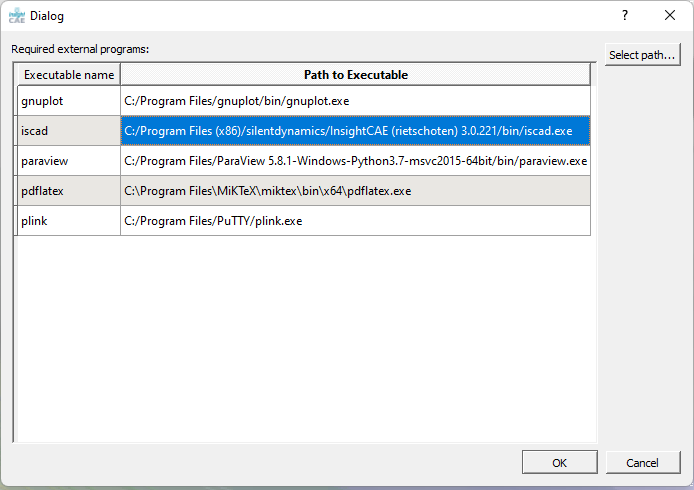
\includegraphics[width=0.5\textwidth]{figs/workbench/set_paths}
\caption{Configuration dialog to set the paths to commonly used third party executables}
\label{fig:set_paths}
\end{figure}

\begin{figure}[ht]
\centering
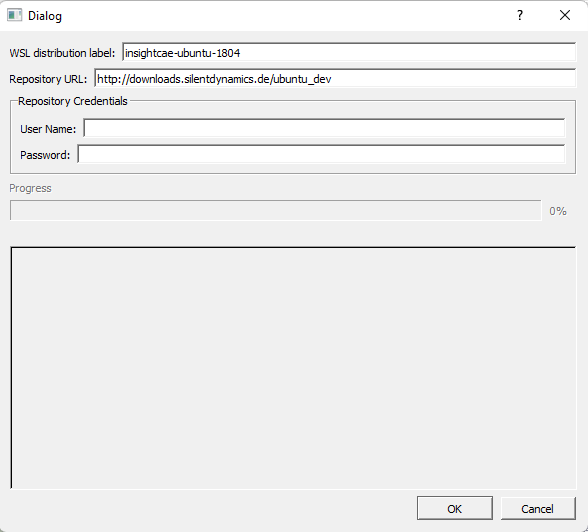
\includegraphics[width=0.7\textwidth]{figs/workbench/create_wsl}
\caption{Create WSL backend form}
\label{fig:create_wsl}
\end{figure}

\paragraph{Updating}

To update to a newer version, just download the newer installer from the location described above and execute it.

Only the last component (InsightCAE) needs to be checked in the installation wizard.
If the third party tools were already installed, they may be skipped.

On the first launch of the workbench after the update is done, the version of the WSL backend(s) is checked.
They will now be different than that of the updated workbench and it is offered to trigger an update.
This should be done since it is important to keep the versions of the frontend and the backend equal.

When the backend update is started, a log window appears and shows the output of the update command.
The update takes several minutes since the updated package will be downloaded and unpacked. 
It is finished when the message "=== Update finished ===" appears in the log.

\subsection{Building from Sources}

\subsubsection{Getting the Source Code}

The source code of InsightCAE is hosted at Github. 
Cloning a working copy constitutes the best way to get updates and the latest bug fixes.

Alternatively, you can download snapshot archives from github, if you don't want to bother with a git client.
In this case, just replace the cloning step below with unpacking the archive.

First, get the the sources by cloning the git repository:
\begin{lstlisting}[language=bash]
$ git clone https://github.com/hkroeger/insightcae.git insight-src
\end{lstlisting}


\subsubsection{Dependencies}

The InsightCAE project depends on a number of other projects.
Some of the dependencies are optional and only required, if certain features are enabled.
The dependencies are listed in table \ref{tab:dependencies}.

\begin{table}[h!]
\centering
\begin{tabular}{lll}
\hline
Project & tested version & required for\\
\hline

Armadillo & 9.800.4 & (always)\\
Gnu Scientific Library & 2.6 & (always)\\
Boost & 1.65.1 &(always) \\
VTK & 9 & (always)\\
Python (Lib) & 3.6 & (always)\\
OpenCASCADE & 7.4 & (always)\\
DXFlib & 3.7.5 & (always)\\
libpoppler & 0.86 & (always) \\
Qt & 5.15 & for GUIs\\
Gmsh & 4.8 & only for analyses with tet/tri meshing\\
Wt toolkit & 4.1 & only for client/server execution\\
OpenFOAM & ESI1806, 4.1 extend & only for OpenFOAM based analyses\\
Code\_Aster & 14 & only for FEM analyses \\
SWIG & 4 & only for python bindings \\
\hline
\end{tabular}
\caption{Required dependencies for building InsightCAE}
\label{tab:dependencies}
\end{table}

\subsubsection{Building}


CMake is utilized for managing the build. 
The preferred way is to build the software out of source in a separate build directory. Create a build directory, then configure the build using e.g. ccmake and finally build using make:

\begin{lstlisting}[language=bash]
$ mkdir insight && cd insight
$ ccmake ../insight-src
\end{lstlisting}
In the CMake GUI, you may need to change paths or adapt settings. Please refer to the CMake documentation\footnote{\url{https://cmake.org/cmake/help/latest/guide/tutorial/index.html}} on how to use CMake.
The biggest difficulty will probably be, to provide all the software packages, on which InsightCAE depends.

The final step in CMake is, to generate the Makefiles. Once this is done without errors, start the compilation of the project by executing:

\begin{lstlisting}[language=bash]
$ make
\end{lstlisting}

To work with InsightCAE, some environment variables are needed to be set up. A script is provided therefore. It can be parsed e.g. in your \file{\textasciitilde/.bashrc} script by adding to the end:

\begin{lstlisting}[language=bash]
source /path/to/insight/bin/insight_setenv.sh
\end{lstlisting}



\subsection{Setting up the Environment}
\label{sec:setupenvironment}

To set up the environment variables and search paths required by the InsightCAE components, a script needs to be parsed.
This is conveniently added to the shell startup script file \file{\textasciitilde/.bashrc}.
Add the following line to the \emph{beginning} of the \file{\textasciitilde/.bashrc} file:

\begin{lstlisting}
source /opt/insightcae/bin/insight_setenv.sh
\end{lstlisting}

Note that the default contents of this file differs between linux distributions.
Sometimes it contains statements which prematurely end its evaluation for non-interactive shells.
This